\section{Problem 2: Einstein Solid}

\subsection{Results}

\subsubsection{Numerical and Analytical Heat Capacity}
%
The numerical and analytical Einstein heat capacities are shown in Fig. (\ref{einstein_numerical_and_analytical_heat_capacities}). Across the temperature range 0.1 to 2000 K, the numerical heat capacities show strong agreement with their analytical counterparts.
\begin{figure}[h]
    \centering
    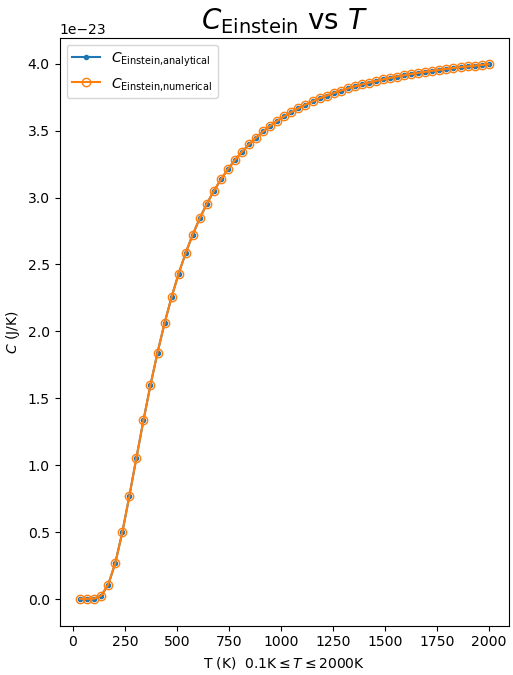
\includegraphics[width=9cm]{einstein_numerical_and_analytical_heat_capacities.png}
    \caption{Numerical and Analytical Einstein Heat Capacity vs Temperature}
    \label{einstein_numerical_and_analytical_heat_capacities}
\end{figure}
\begin{table}[h]
\begin{center}
    \begin{tabular}{|c|c|c|}
        \hline
        \textbf{System Parameter} & \textbf{Value} & \textbf{Notes} \\ \hline
        No. of Atom(s) & 1 & - \\ \hline
        Einstein Frequency & 1.728$\times 10^{14}$ s$^{-1}$ & for Diamond, from Simon \cite[page 13]{Simon2013} \\ \hline
        Finite Difference Magnitude ($\Delta T$) & 0.001 K & arbitrary \\ \hline
    \end{tabular}
\end{center}
\caption{System Parameters for Einstein Heat Capacity}
\label{system_parameters_for_Einstein_heat_capacity}
\end{table}

\subsection{Discussion}

The Einstein solid modeled in this section takes in the energy spectrum of the quantum harmonic oscillator modeled in the previous section as its input for calculating internal energy and heat capacity.